\begin{figure}[h]
	\caption{An example of a bar chart}
	\medskip
	\pgfplotsset{compat=newest}
	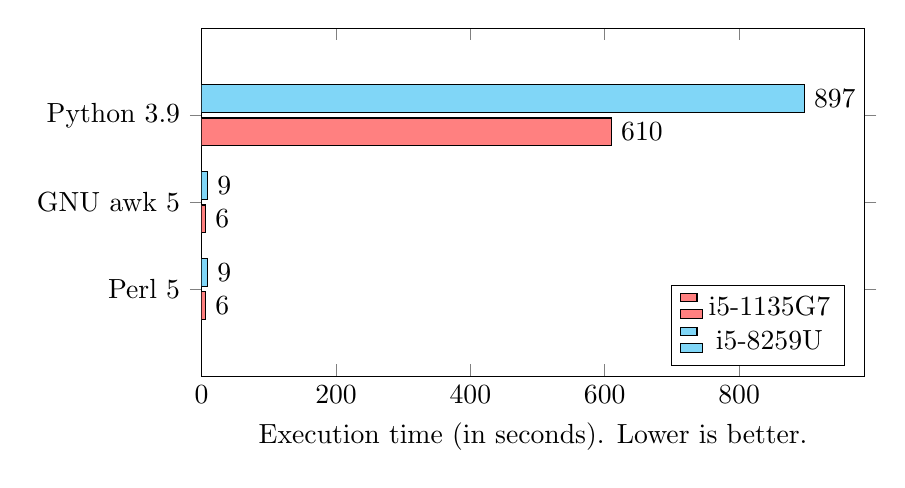
\begin{tikzpicture}
		\begin{axis}
			[ 
			xbar, 
			xmin=0, 
			width=10cm,
			height=6cm, 
			enlarge y limits=0.5, 
			xlabel={Execution time (in seconds). Lower is better.},
			%ylabel={Language},
			symbolic y coords={perl,gawk,python}, 
			yticklabels={Python 3.9,GNU awk 5,Perl 5},
			ytick=data,
			nodes near coords,
			nodes near coords align={horizontal}, 
			legend pos=south east
			]
			\addplot[fill=red!50] coordinates {(610,python) (6,gawk) (6,perl)}; 
			\addplot[fill=cyan!50] coordinates {(897,python) (9,gawk) (9,perl)};
			\legend{i5-1135G7,i5-8259U};
		\end{axis} 
	\end{tikzpicture}
\end{figure}
